%% Multi-Site Calibration of Volcanic Sedimentation Rates in Java
%% JASREP v3.0 — Path B narrow-scope rewrite (Mata Elang #15, 2026-04-20)
%% v2.0 -> v3.0 changes: removed demographic null (§2.2 last paragraphs),
%%   West Java comparandum (§2.5), five-factor cascade (§5.5), Kutai full argument
%%   (§5.4). Those arguments relocated to P0 "The Invisible Civilization" synthesis.
%%   Added: compaction, erosion, spatial autocorrelation, monument-vs-settlement
%%   caveats in §5.6 per critical review 2026-04-20.
%% Target: ~15-18 pp single-identity geoarchaeology paper.
%% Submission route: subscription (zero APC). Target: JASREP (Elsevier Q1).

\documentclass[12pt,a4paper]{article}
\usepackage[utf8]{inputenc}
\usepackage[T1]{fontenc}
\usepackage{graphicx}
\usepackage{amsmath}
\usepackage{natbib}
\usepackage{booktabs}
\usepackage{hyperref}
\usepackage[left=2.5cm,right=2.5cm,top=2.5cm,bottom=2.5cm]{geometry}
\usepackage{lineno}
\usepackage{setspace}
\doublespacing
\linenumbers

\begin{document}

\title{Multi-Site Calibration of Volcanic Sedimentation Rates and Implications for Archaeological Visibility in Java, Indonesia}

\author{Mukhlis Amien\textsuperscript{1,*} \and Go Frendi Gunawan\textsuperscript{1}}

\date{}

\maketitle

\noindent\textsuperscript{1}Lab Data Sains, Universitas Bhinneka Nusantara, Malang, Indonesia\\
\textsuperscript{*}Correspondence: amien@ubhinus.ac.id

\begin{abstract}
Java hosts 45 active volcanoes in 129,000~km\textsuperscript{2}, and its archaeological record becomes progressively sparser with age in the volcanic interior. We ask a narrowly geomorphological question: at what rate has cumulative volcanic sedimentation buried the landscape, and what does that rate imply for the detection horizon of surface survey?

In 1803, the Dutch colonial administrator Nicolaus Engelhard documented two stone guardian statues at Candi Singosari in East Java---each 370~cm tall, carved from monolithic andesite in 1268~CE---with approximately half their bodies below ground. Gunung Kelud had erupted about twenty times in the intervening 535 years, and the landscape had risen around them at approximately 3.5~mm per year. We extend this inference with three additional calibration sites from the Merapi system in Central Java, establishing a mean cumulative aggradation rate of $4.4 \pm 1.2$~mm/yr across two volcanic systems and 350~km of Java. The cross-system convergence is the central finding.

Applied as a first-order linear projection, this rate places Kanjuruhan-era (\textasciitilde760~CE) deposits at 3.0--7.9~m and pre-400~CE deposits at 3.9--10.1~m depth in the Malang basin---exceeding conventional surface survey and approaching the upper limit of ground-penetrating radar in volcanic sediment. A 51-pair eruption--site dataset compiled independently from colonial and volcanological literature yields a mean measured depth of 3.41~m, consistent with the rate model over a 760-year horizon. Spatial analysis of 666 East Java sites shows near-volcano clustering that reflects survey intensity and monument durability rather than settlement distribution. We present the calibration as a methodological foundation for targeted subsurface investigation in Java's volcanic terrain.

\medskip
\noindent\textbf{Keywords:} volcanic taphonomy; cumulative sedimentation; detection horizon; East Java; multi-site calibration; geoarchaeology
\end{abstract}


\section{Introduction}

In 1803, a Dutch colonial administrator named Nicolaus Engelhard encountered something at the ruins of Candi Singosari that has not received the theoretical attention it deserves. Two enormous stone guardian statues---\textit{Dwarapala}, each 370~cm tall and carved from a single block of andesite---stood with roughly half their bodies below the ground. They had been installed in 1268~CE, during the reign of King Kertanegara of the Singosari kingdom \citep{kinney2003}. The ground had risen around them at approximately 3.5~mm per year, driven by 535 years of repeated eruptions from Gunung Kelud, 35~km to the east. Only their scale made them visible at all.

Hindu-Buddhist kingdoms flourished on Java from at least the 4th century~CE, yet the material record of the earliest Javanese polities is comparatively sparse. Stone temples of the 8th to 15th centuries survive because they are monumental; organic architecture does not. This paper does not attempt to reconstruct what the pre-monumental record looked like---that question is taken up in a companion synthesis (Amien, in preparation). Here the scope is narrower: to quantify the rate at which cumulative volcanic sedimentation has buried the Javanese landscape, and to evaluate what that rate implies for the depth at which historical-era deposits now reside.

The mechanism at work is not the catastrophic burial familiar from Pompeii, Akrotiri, or Cer\'{e}n---single eruptions sealing settlements in hours \citep{sigurdsson1985,doumas1983,sheets1992}. It is \textit{cumulative} sedimentation: repeated small eruptions depositing millimeters per event, accumulating to meters over centuries (Sect.~2.3). In Java, every point on the island lies within approximately 27~km of an active vent \citep{vanbemmelen1949}, placing the entire landmass within the depositional range of at least one volcanic center. The Dwarapala statues provide direct photographic documentation of this process at a known, measurable rate (Fig.~\ref{fig:dwarapala_photos}).

\begin{figure*}[t]
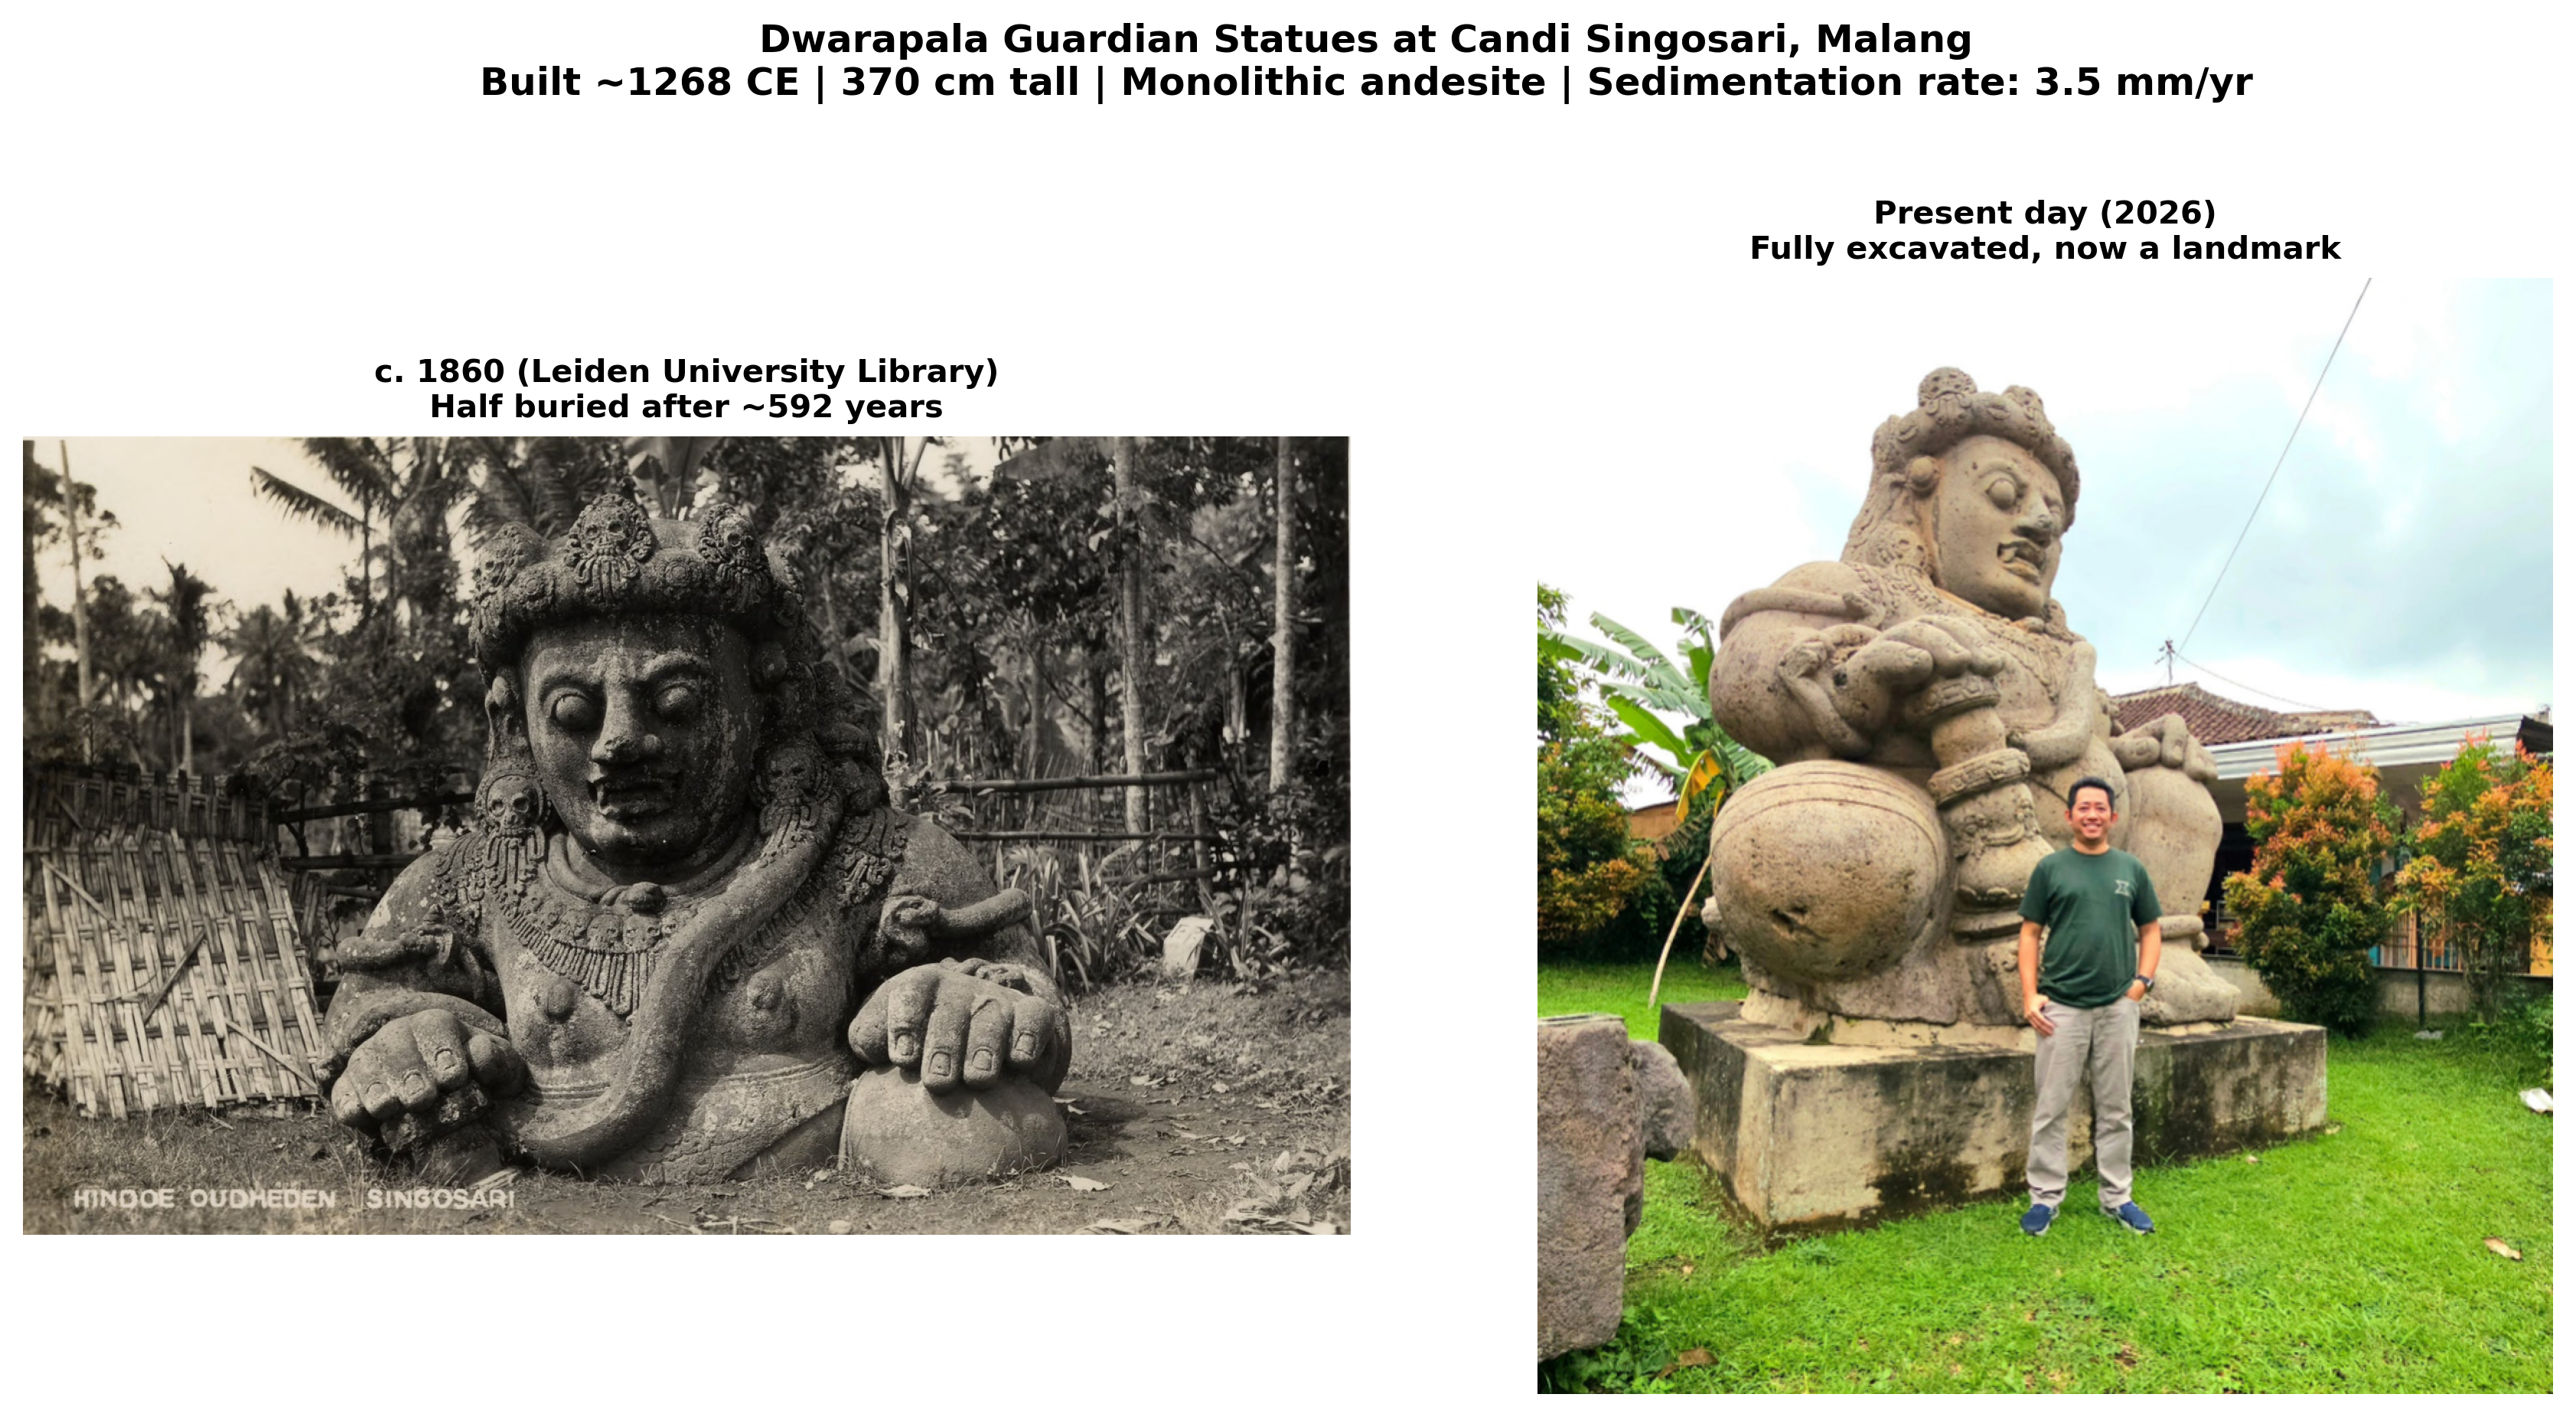
\includegraphics[width=12cm]{figures/fig0_dwarapala_comparison.png}
\caption{Dwarapala guardian statues at Candi Singosari, Malang, East Java. Left: colonial-era photograph (c.~1860) from the Leiden University Library archives, showing the statue partially buried beneath volcanic sediment---only the head, shoulders, and hands remain visible above the accumulated overburden. Right: present-day condition after excavation, revealing the full 370~cm height. The statues were constructed \textasciitilde1268~CE during the reign of Kertanegara; approximately 185~cm of volcanic overburden accumulated by their rediscovery in 1803~CE, yielding a calibrated sedimentation rate of 3.5~mm/yr (Sect.~3.2).}
\label{fig:dwarapala_photos}
\end{figure*}

Surface visibility is a recognized problem in archaeological survey \citep{wandsnider1992,french2003}, but its implications for volcanic landscapes in island Southeast Asia have been largely unexplored. Research in the region has focused on monumental stone architecture---the class of evidence most resistant to burial \citep{degroot2009}---producing an inherent circularity: stone temples are found because they protrude through sediment; their distribution is interpreted as reflecting settlement patterns; and the wooden settlements that constituted the overwhelming majority of historical habitation are overlooked entirely.

The empirical foundation of this study is a four-site calibration. We compiled construction dates and measured burial depths for four archaeological sites: the Dwarapala statues at Candi Singosari (\textasciitilde1268~CE, Kelud volcanic system) and three Hindu-Buddhist temples near Merapi in Central Java (Sambisari, Kedulan, and Kimpulan, all 9th century~CE). These span roughly 350~km of Java and two geologically distinct volcanic systems. Kelud has produced 37 confirmed eruptions since 1000~CE \citep{gvp2024}. Merapi is one of the world's most persistently active stratovolcanoes \citep{gertisser2012}. The sedimentation rates converge within a factor of two---a finding that was not guaranteed and that we consider central to the argument.

Those rates are applied to project burial depths for successive historical periods: Kanjuruhan-era (\textasciitilde760~CE) remains in the Malang basin are predicted to lie at 3.0--7.9~m---exceeding the reach of surface survey and approaching the upper limit of ground-penetrating radar in volcanic sediment \citep{putra2019,conyers2004}. A spatial analysis of 666 known archaeological sites in East Java is included for descriptive context rather than as a test of the calibration: the distribution is shaped by both survivorship (monumental stone versus organic architecture) and two centuries of survey concentrated on the Singosari--Majapahit heartland, and cannot by itself confirm or refute a taphonomic interpretation.


\section{Background}

\subsection{Java as a volcanic burial zone}

Java hosts 45 active volcanoes across approximately 129,000~km\textsuperscript{2}---a volcanic density of 0.35 per 1,000~km\textsuperscript{2}, the highest of any major Indonesian island and approximately six times that of Sumatra (0.06/1,000~km\textsuperscript{2}) \citep{vanbemmelen1949}. The average spacing between volcanic centers is approximately 54~km, meaning that no point on Java lies more than approximately 27~km from the nearest active volcano. Since tephra from VEI~3--4 eruptions can deposit measurable ash at 50--100+~km from the source \citep{newhall1982}, the entire island falls within the depositional range of at least one---and typically multiple---volcanic centers. The relevant archaeological question is therefore not whether volcanic sedimentation occurs at a given location, but how much has accumulated since a site was occupied---a function of distance from active vents, local topography, and eruption history.

East Java province alone encompasses seven major active centers: Kelud, Semeru, Arjuno-Welirang, Bromo, Lamongan, Raung, and Ijen. The Brantas River basin---which hosted the Singosari (1222--1293~CE) and Majapahit (1293--\textasciitilde1500~CE) kingdoms---sits in the depositional path of Kelud (35~km east), Arjuno-Welirang (25~km north), and Semeru (60~km southeast). Kelud alone has produced 37 confirmed eruptions since 1000~CE \citep{gvp2024,maeno2019}.

In Central Java, Mount Merapi---one of the world's most active stratovolcanoes---has buried a cluster of 9th-century Hindu-Buddhist temples to depths of 3--7~m \citep{lavigne2000,thouret2000}. These buried temples (Sambisari, Kedulan, Kimpulan) were discovered accidentally during modern construction and mining activities, not through systematic archaeological survey.

\subsection{The observable archaeological record in East Java}

Our compilation of known archaeological sites in East Java (Sect.~3.1) identified 666 unique entries, of which only 391 (59\%) have usable spatial coordinates. The dataset is dominated by stone monuments (\textit{candi}) from the Singosari and Majapahit periods (13th--15th centuries~CE) \citep{kinney2003}. Earlier periods are poorly represented: pre-10th century sites constitute less than 5\% of the geocoded total.

This temporal distribution reflects two complementary pressures. Survey has historically concentrated on the Singosari-Majapahit heartland around Blitar, Malang, and Mojokerto. Simultaneously, older sites have accumulated more volcanic overburden and are therefore less likely to be exposed at the modern ground surface. The broader question of whether the pre-10th century absence reflects low population, non-monumental material culture, or taphonomic erasure is taken up in a companion synthesis (Amien, in preparation); the present paper addresses only the geophysical rate at which cumulative sedimentation proceeds.

\subsection{Volcanic taphonomy}

The volcanological literature on archaeological burial is dominated by catastrophic events: Pompeii sealed in eighteen hours, Candi Sambisari buried over roughly a thousand years. These are fundamentally different processes that produce different archaeological signatures.

Catastrophic volcanic burial---a single eruption sealing an entire settlement in hours---is well documented \citep{sigurdsson1985,doumas1983,sheets1992} and, precisely because it is dramatic, attracts sustained excavation attention. \textit{Cumulative} volcanic burial, by contrast, generates no single event to excavate. Ash arrives in centimeters per eruption, lahars rework it downslope, and every decade the ground surface is fractionally higher than the decade before. After five centuries, a surface that was once at ground level lies two meters underground. After fifteen centuries, it may lie at six meters depth. No emergency response is triggered; no excavation follows. The site becomes, gradually and completely, invisible to surface survey.

\subsection{A note on comparative context}

Two observations from elsewhere in the archipelago inform the calibration without being part of its argument. First, the oldest conventionally recognised Indonesian polity, Kutai Martadipura (\textasciitilde400~CE) in East Kalimantan, is known from inscribed stone pillars found near the present ground surface in a region with zero active volcanoes \citep{vogel1918,coedes1968,miksic2004}. Second, three Hindu-Buddhist temples on the Merapi flank (Sambisari, Kedulan, Kimpulan) were discovered beneath 3--7~m of volcanic sediment. These observations bracket the range of outcomes the calibration needs to explain: very shallow burial where no volcanism operates, meter-scale burial where it does. Whether the volcanic/non-volcanic contrast has broader interpretive implications for Indonesian historiography is a question beyond the scope of this paper \citep[see][]{amien_synthesis_forthcoming}.


\section{Data and Methods}

\subsection{Archaeological site dataset}

We compiled a database of known archaeological sites in East Java province from three complementary sources. First, we queried the OpenStreetMap Overpass API for all features tagged with \texttt{historic=*} within the Jawa Timur administrative boundary (bounding box: 6.5--9.0\textdegree{}S, 111.0--115.0\textdegree{}E), yielding 281 geolocated features. Second, we queried the Wikidata SPARQL endpoint for entities with coordinate property P625 within the same bounding box, recovering 16 precisely located sites. Third, we scraped the Indonesian-language Wikipedia article ``Daftar candi di Indonesia'' for 369 additional entries.

To increase spatial coverage, we geocoded the 369 coordinate-less entries using the OpenStreetMap Nominatim API with progressive query refinement. Of 369 queries, 94 returned valid coordinates within the study area (25.5\% success rate). After spatial deduplication within a 100~m radius, the final dataset contains 666 unique site entries, of which 391 have usable coordinates (58.7\% geocoding rate). Within the East Java analytical bounds, 383 geocoded sites were used for spatial analysis.

It should be noted that this dataset is heavily biased toward stone monuments (\textit{candi}) that survived volcanic burial due to their monumental scale. Wooden settlements, which likely constituted the vast majority of historical habitation, are systematically absent---precisely the pattern predicted by the taphonomic bias hypothesis.

\subsection{The Dwarapala calibration}

The primary empirical anchor for the burial depth framework is the pair of Dwarapala guardian statues at Candi Singosari, Malang Regency, East Java. The statues were constructed approximately 1268~CE during the reign of Kertanegara of the Singosari Kingdom and discovered in 1803~CE by the Dutch colonial administrator Nicolaus Engelhard. Each statue stands 370~cm in seated height and weighs approximately 40 tonnes, carved from monolithic andesite. At the time of discovery, approximately half of each statue's body was below the ground surface (``\textit{separuh tubuh terpendam}''), corresponding to an estimated burial depth of approximately 185~cm accumulated over 535 years (1803 $-$ 1268 = 535 years). The resulting sedimentation rate is:

\begin{equation}
  R = \frac{185~\text{cm}}{535~\text{yr}} = 0.35~\text{cm/yr} = 3.5~\text{mm/yr}
\end{equation}

This rate is internally consistent with the documented eruption history of Gunung Kelud. The volcano erupted approximately 20 times between 1268 and 1803~CE, and documented VEI~3--4 eruptions deposit 2--20~cm of ash at the distance of Malang (\textasciitilde35~km from the vent). Twenty eruptions at an average of approximately 5~cm per event would account for approximately 100~cm of the 185~cm total burial. The remainder (\textasciitilde85~cm) is attributable to secondary remobilization (lahars, reworked tephra), contributions from the Semeru and Arjuno-Welirang volcanic systems, and non-volcanic aggradation \citep{gvp2024,maeno2019}. The rates reported here represent \textit{total landscape aggradation} in volcanic terrain, not pure primary tephra accumulation; for archaeological burial, however, the total aggradation rate is the operationally relevant metric regardless of depositional source.

The Dwarapala burial timeline from construction to present is illustrated in Fig.~\ref{fig:timeline}.

\begin{figure}[t]
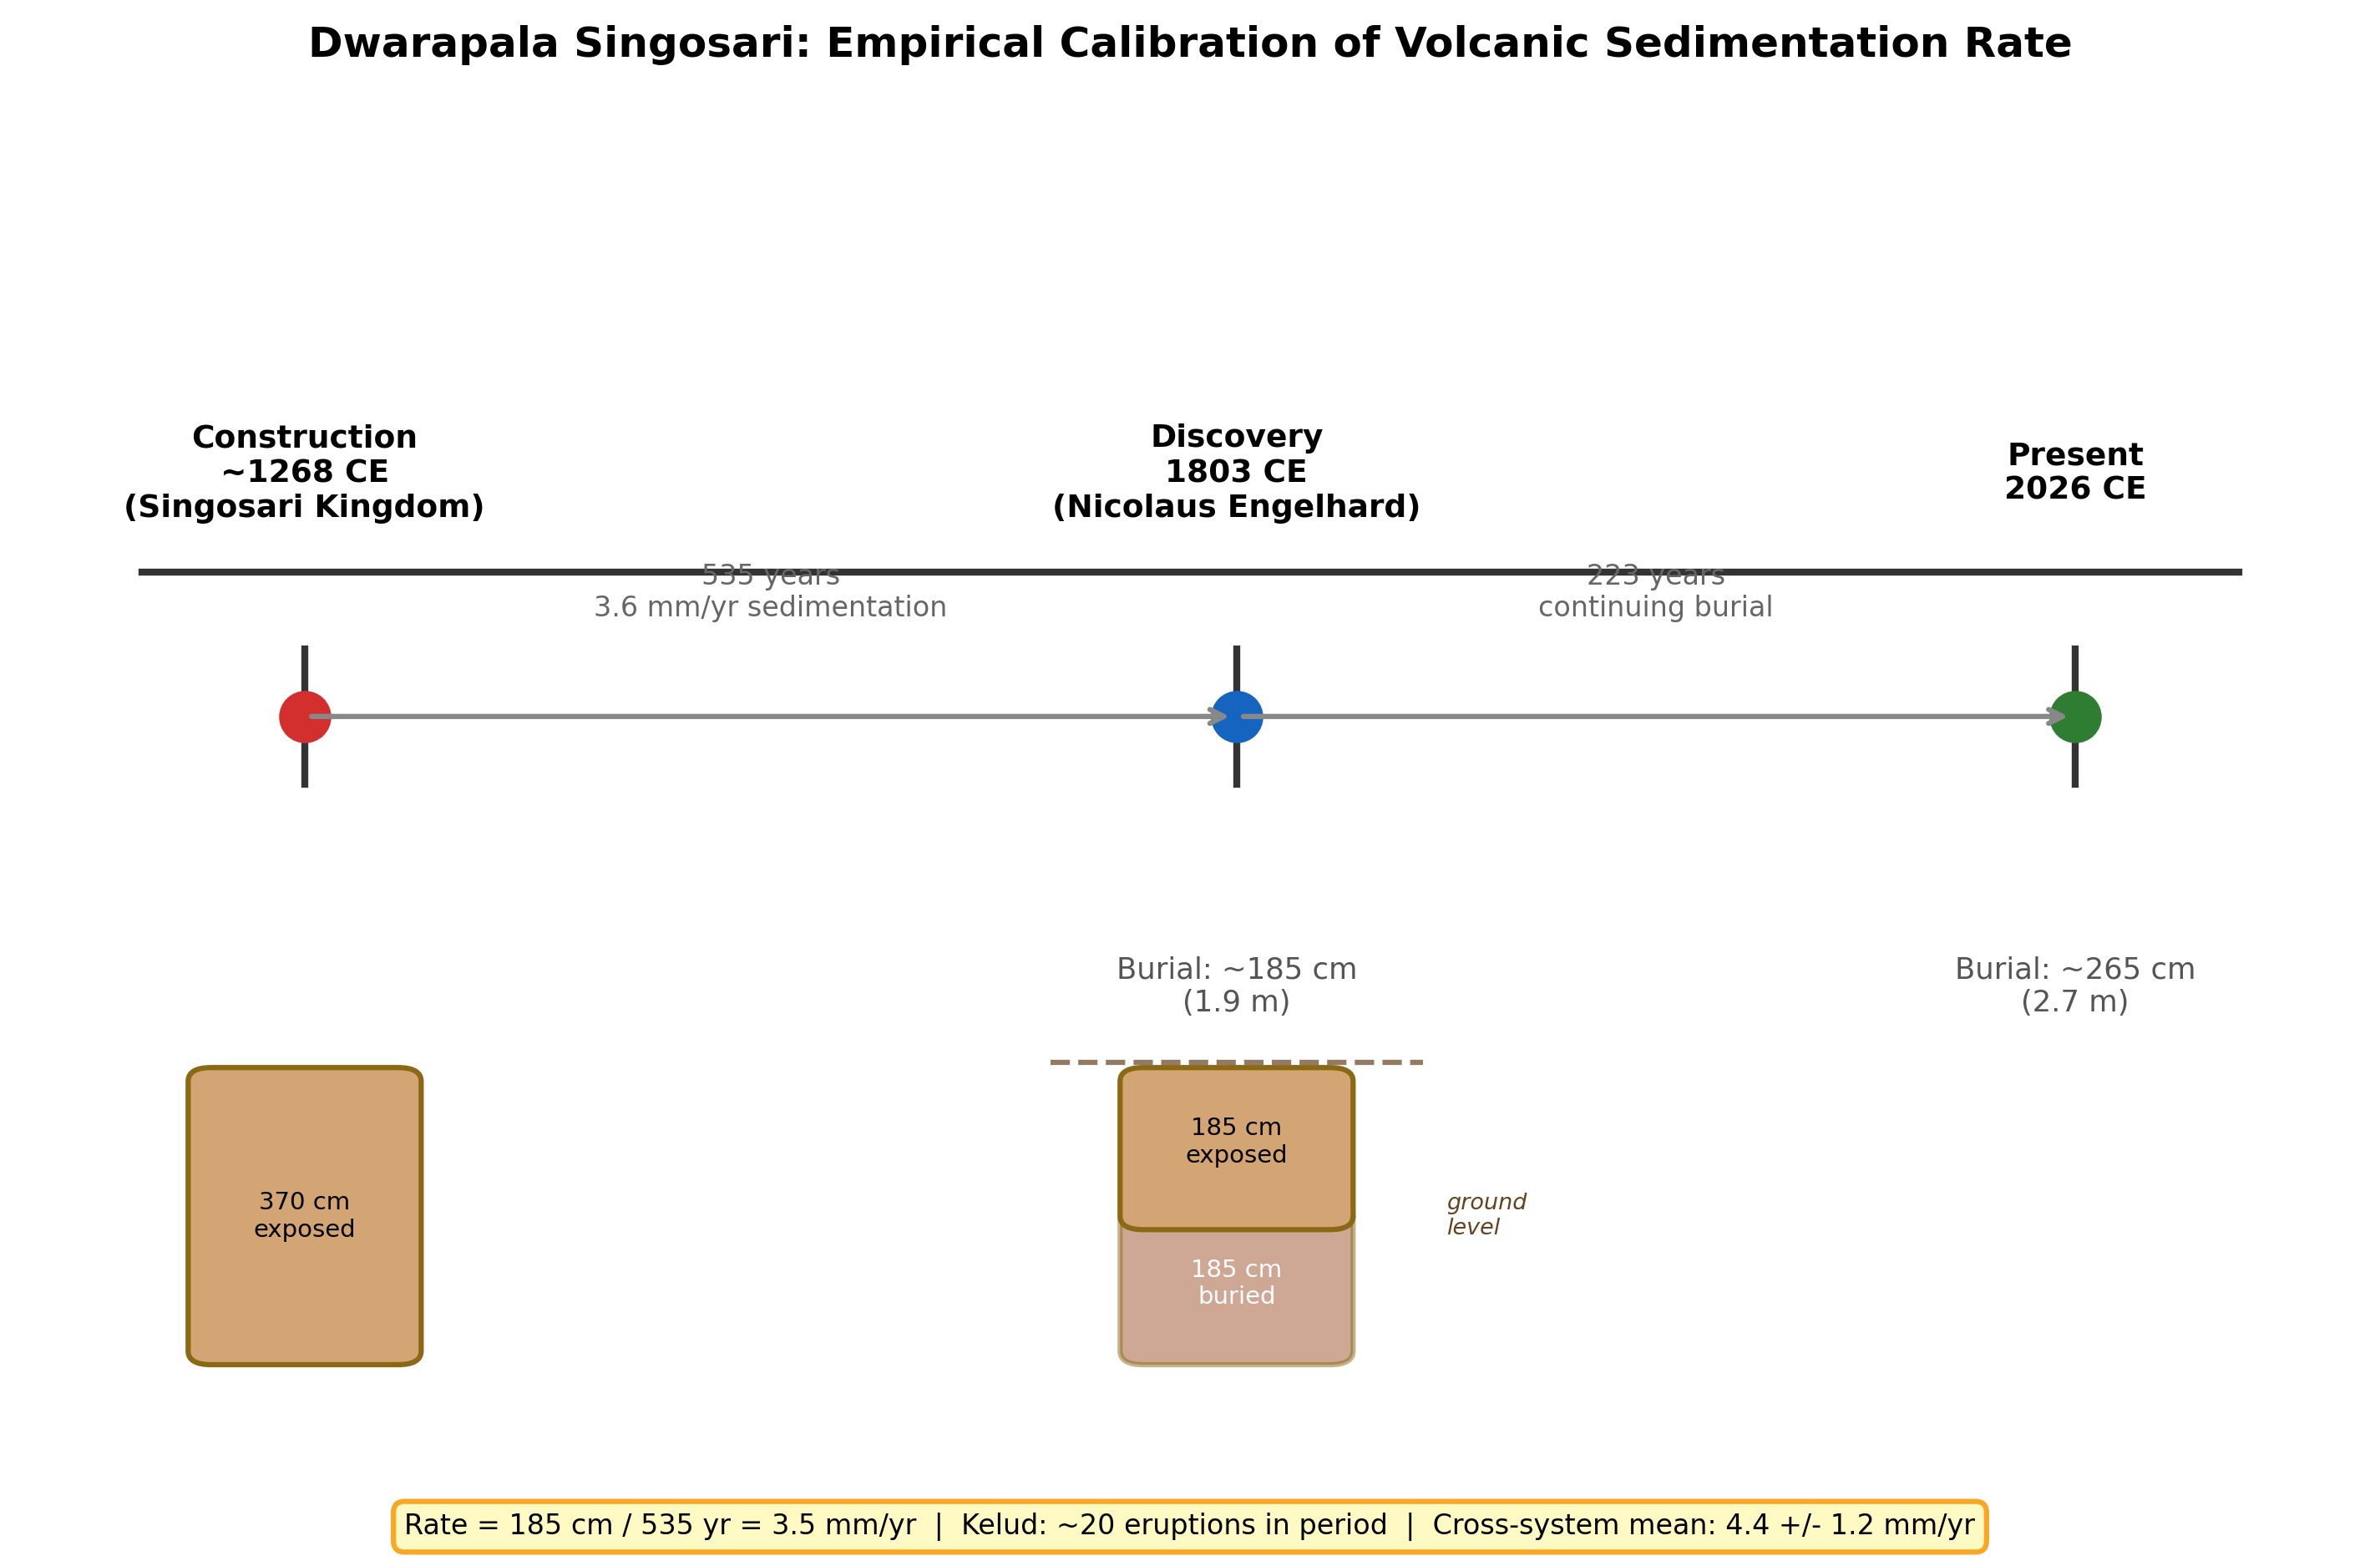
\includegraphics[width=8.3cm]{figures/fig1_dwarapala_timeline.png}
\caption{Dwarapala Singosari burial timeline. The statues were constructed \textasciitilde1268~CE at full height (370~cm) and discovered in 1803~CE with approximately half (185~cm) buried by volcanic sedimentation, yielding a cumulative rate of 3.5~mm/yr. The cross-system mean from four calibration points is $4.4 \pm 1.2$~mm/yr.}
\label{fig:timeline}
\end{figure}

\subsection{Secondary calibration points}

To assess whether the Dwarapala rate is a local anomaly or representative of a Java-wide phenomenon, we compiled three additional calibration points from Central Java's Merapi volcanic system (Table~\ref{tab:calibration}).

\begin{table}[t]
\caption{Empirical calibration points for volcanic sedimentation rates at archaeological sites in Java. BPCB-Jatim and BPCB-DIY are Indonesia's regional heritage conservation agencies (\textit{Balai Pelestarian Cagar Budaya}, Ministry of Education and Culture); burial depths are from their published excavation reports. Sambisari and Kedulan depths are cited in \citet{lavigne2000} and \citet{thouret2000}.}
\label{tab:calibration}
\begin{tabular}{lcccccc}
\toprule
Site & Built (CE) & Discovered & Depth (cm) & System & Rate (mm/yr) & Source \\
\midrule
Dwarapala Singosari & \textasciitilde1268 & 1803 & \textasciitilde185 & Kelud & 3.5 & BPCB Jatim \\
Candi Sambisari & \textasciitilde835 & 1966 & 500--650 & Merapi & 4.4--5.7 & BPCB DIY \\
Candi Kedulan & \textasciitilde869 & 1993 & 600--700 & Merapi & 5.3--6.2 & BPCB DIY \\
Candi Kimpulan & \textasciitilde900 & 2009 & 270--500 & Merapi & 2.4--4.5 & \citet{putra2019} \\
\bottomrule
\end{tabular}
\end{table}

Across all four sites, the computed rates span 2.4--6.2~mm/yr. Taking the midpoint of each site's range (Dwarapala: 3.5; Sambisari: 5.1; Kedulan: 5.8; Kimpulan: 3.5~mm/yr) yields a mean of $4.4 \pm 1.2$~mm/yr (1$\sigma$, $n=4$). The full observed range of 2.4--6.2~mm/yr is used for all subsequent projections. The consistency across two independent volcanic systems---Kelud in East Java and Merapi in Central Java---demonstrates that mm/yr-scale burial of archaeological sites is systematic and Java-wide, not a local anomaly (Fig.~\ref{fig:rates}).

\subsection{Independent validation: eruption--site correlation dataset}

As an independent check on these calibration rates, we compiled a dataset of 51 documented eruption--archaeological site correlations from across 12 volcanic systems in Island Southeast Asia. Sources were historical and colonial-era records documenting specific volcanic events and their effects on specific known sites; 86\% of the evidence was primary (directly observed and recorded, not inferred from proximity). Of the 51 pairs, 24 include physically measured burial depths. The mean measured depth across these 24 sites is 3.41~m (median 2.50~m), consistent with the four-site calibration mean of 4.4~mm/yr applied over a 760-year horizon (expected depth: 3.3~m). This dataset shares no sites with the primary calibration and provides independent confirmation that meter-scale burial is a normal outcome of multi-century volcanic sedimentation at archaeological sites across the region.

\begin{figure}[t]
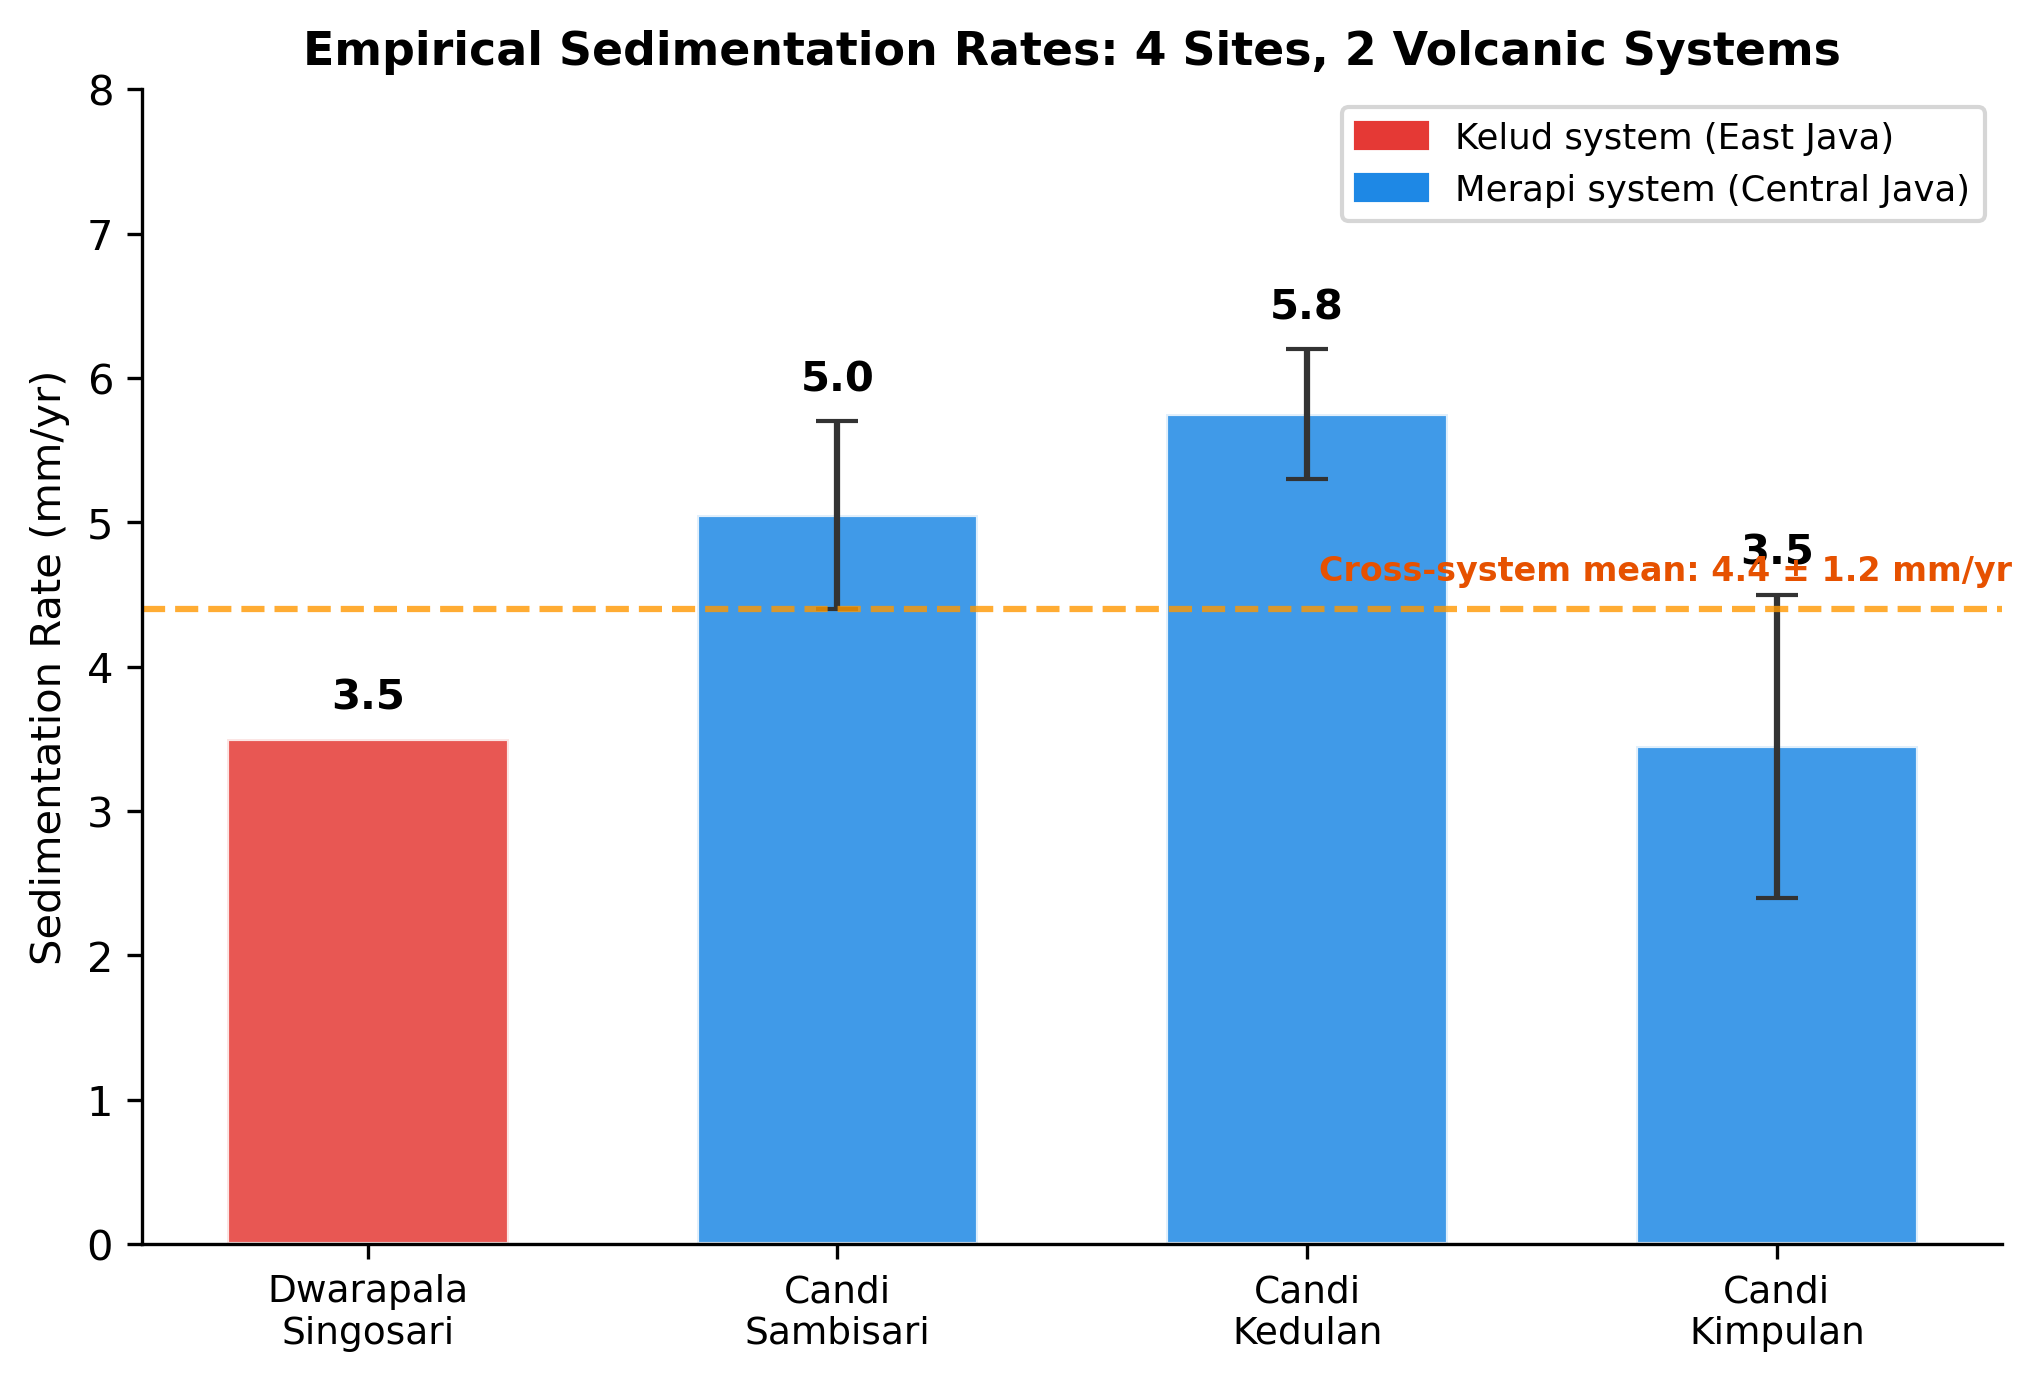
\includegraphics[width=8.3cm]{figures/fig3_calibration_rates.png}
\caption{Empirical sedimentation rates from four archaeological sites across two volcanic systems. Error bars show the range from reported depth uncertainty. The cross-system mean is $4.4 \pm 1.2$~mm/yr.}
\label{fig:rates}
\end{figure}

\subsection{Burial depth projection model}

Using the empirically derived rate range, we estimate expected overburden depth by era according to the linear model:

\begin{equation}
  D(\text{era}) = R \times (T_{\text{present}} - T_{\text{era}})
\end{equation}

\noindent where $R$ ranges from 2.4 to 6.2~mm/yr and $T_{\text{present}} = 2026$~CE. This linear model is a first-order approximation; actual deposition is episodic, with eruption clusters interspersed by quiescent periods and subject to compaction. The wide rate range (2.4--6.2~mm/yr) partially captures this variability. Results are presented in Fig.~\ref{fig:depth}.

\begin{figure*}[t]
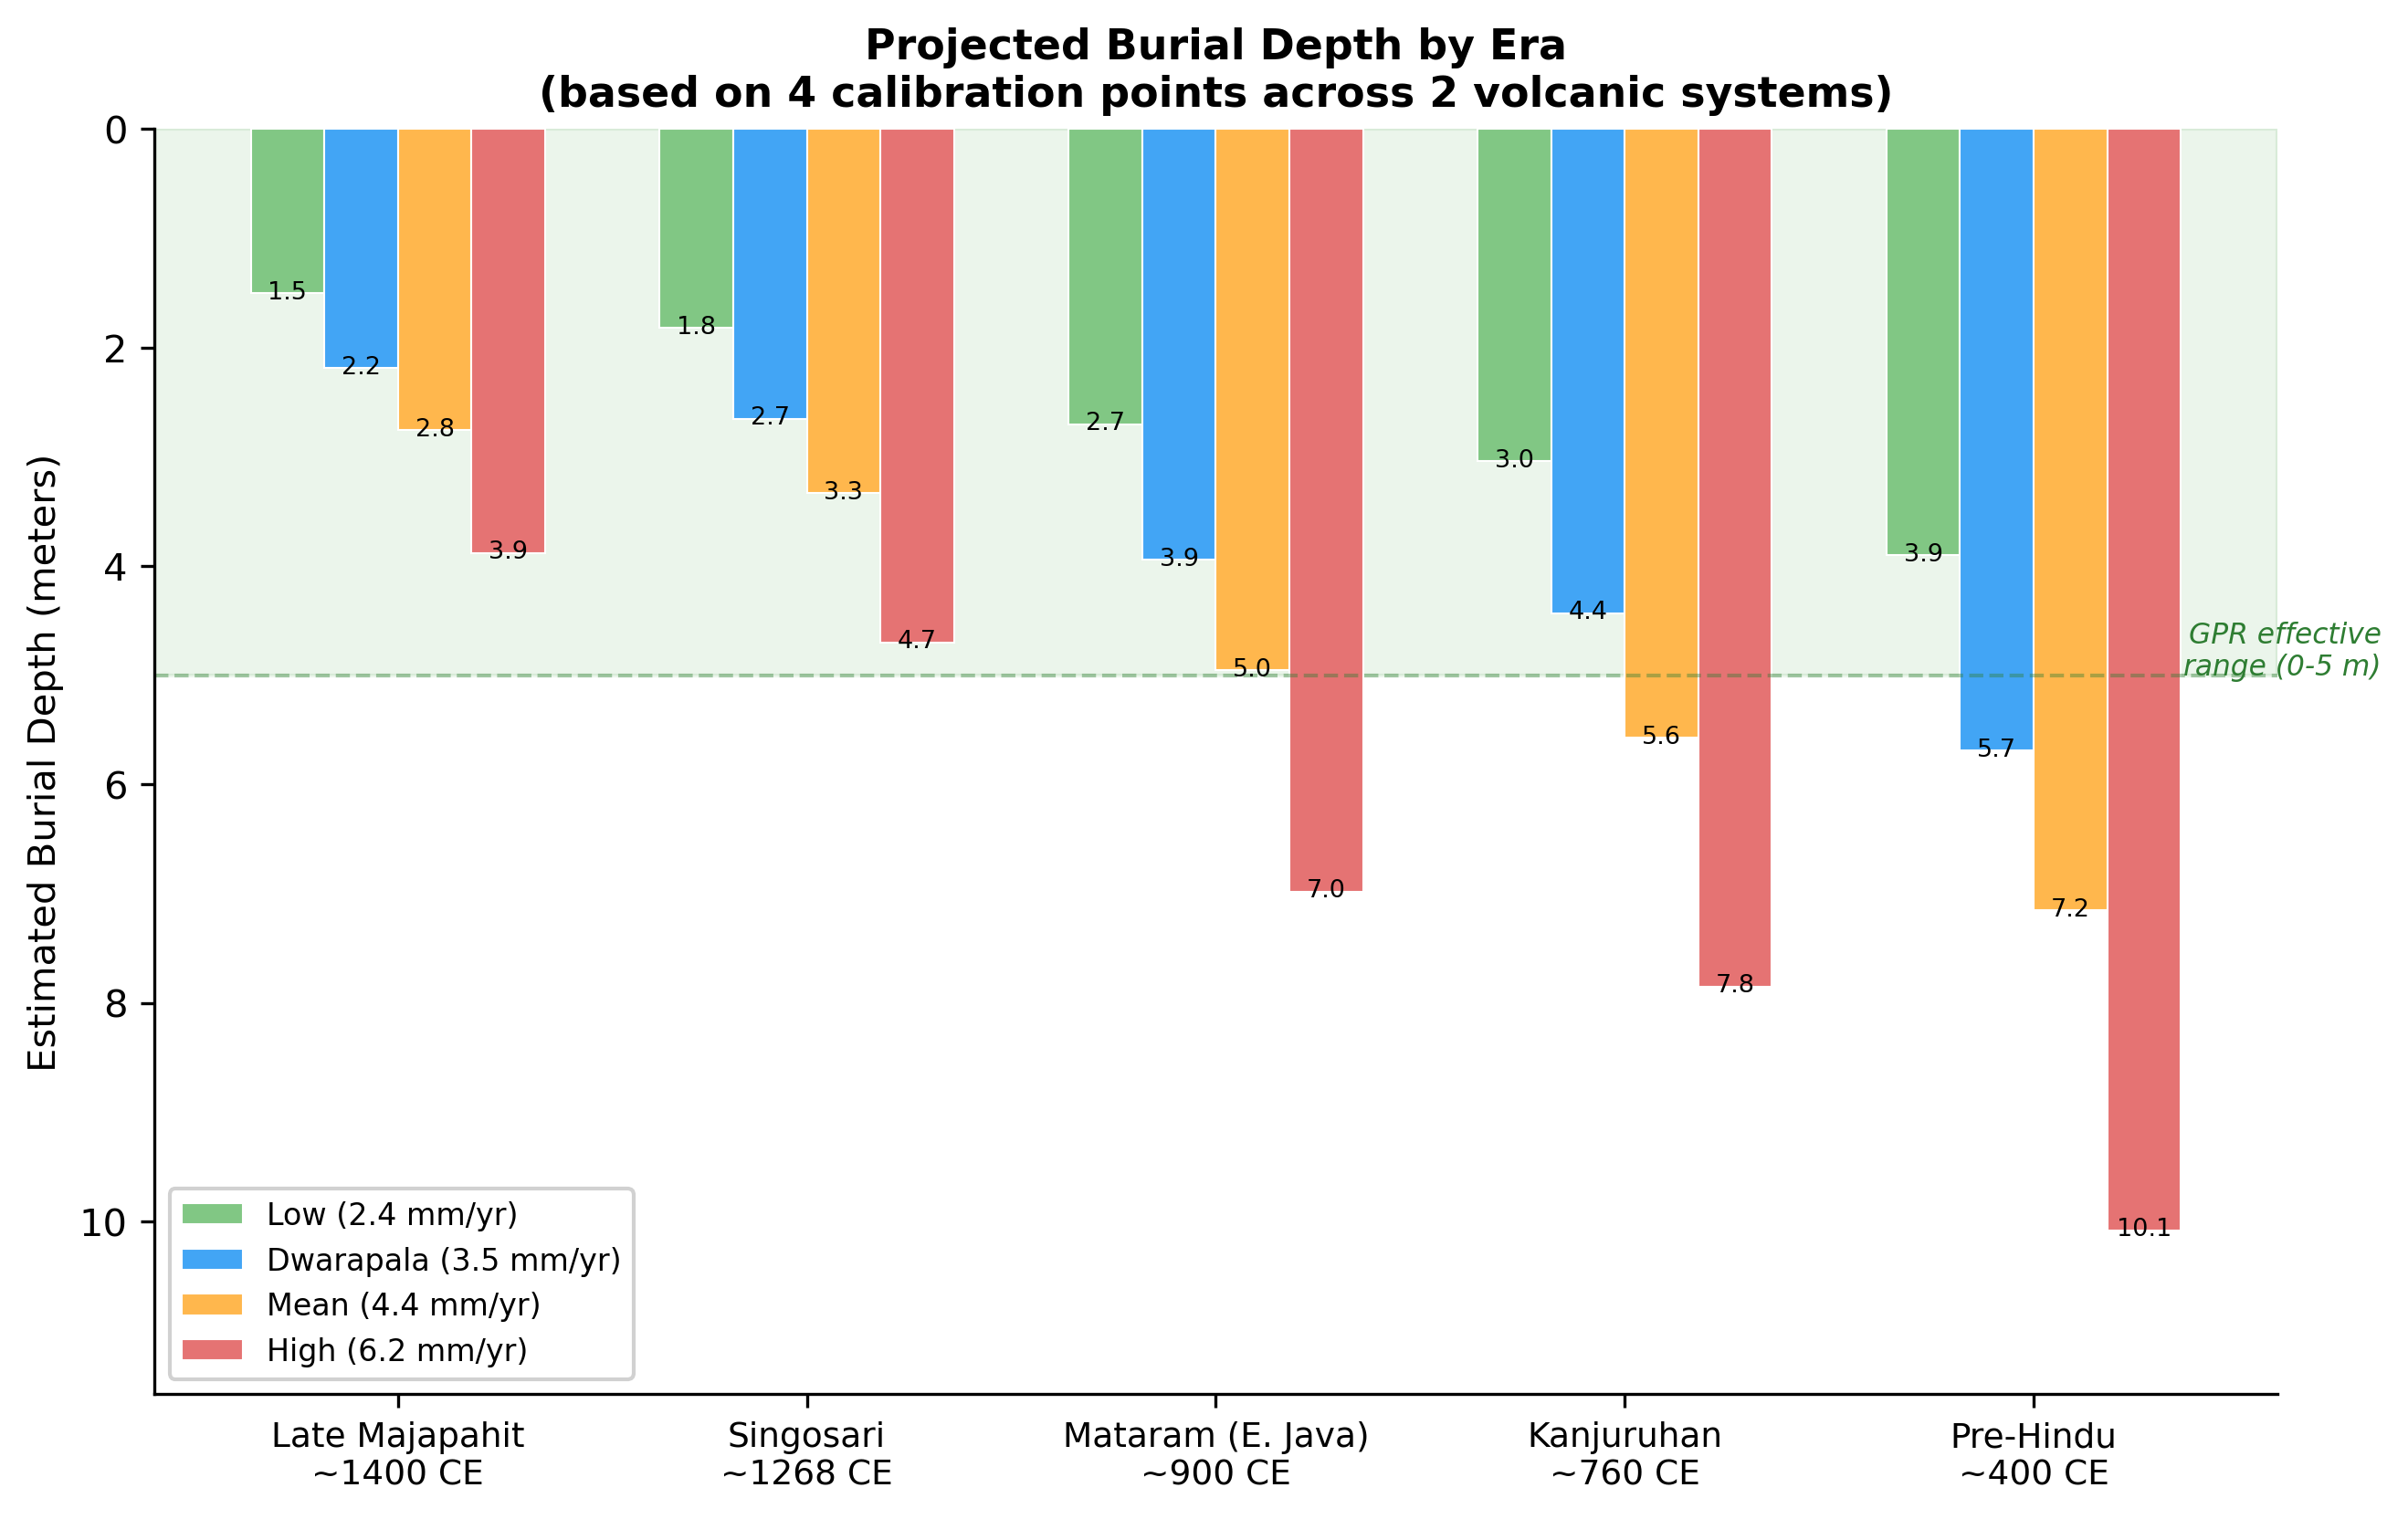
\includegraphics[width=12cm]{figures/fig2_burial_depth_projections.png}
\caption{Projected burial depth by historical era using four empirically-derived sedimentation rates. The green band indicates the effective range of ground-penetrating radar in volcanic sediment (0--5~m). Kanjuruhan-era and earlier remains may exceed GPR detection limits.}
\label{fig:depth}
\end{figure*}

\subsection{Spatial analysis methods}

Two complementary spatial analyses were conducted to examine the relationship between site distribution and volcanic proximity.

In the first analysis, we computed the minimum great-circle distance from each geocoded site to the nearest of seven reference volcanoes. Sites were binned into seven distance bands (0--25, 25--50, 50--75, 75--100, 100--150, 150--200, and 200+~km), and site density was expressed as sites per 1,000~km\textsuperscript{2}. Spearman's rank correlation between distance band midpoint and site density was used to test whether sites are found preferentially near or far from volcanoes.

In the second analysis, we controlled for the effect of terrain suitability on site distribution by constructing a terrain suitability index combining four DEM-derived features: slope, elevation, topographic wetness index (TWI), and a river proximity proxy. The study area was divided into a 25~km $\times$ 25~km grid (187 cells). For each cell, we computed the residual between observed and terrain-predicted site count. Spearman correlation between residual density and distance to the nearest volcano tests the taphonomic bias hypothesis after controlling for terrain preference.


\section{Results}

\subsection{The Dwarapala calibration}

The Dwarapala sedimentation calculation yields a rate of 3.5~mm/year (Sect.~3.2). This rate is internally consistent with documented Kelud eruption histories, which account for approximately 100 of the 185~cm total burial through direct tephra deposition alone. The remaining 85~cm is attributable to secondary remobilization and contributions from other volcanic systems.

The secondary calibration points yield rates of 2.4--6.2~mm/yr across the Merapi system, consistently higher than the Dwarapala rate (3.5~mm/yr) from the Kelud system. This difference is physically plausible: Merapi erupts more frequently than Kelud, and the Central Java sites are closer to their volcanic source. The cross-system mean of $4.4 \pm 1.2$~mm/yr establishes that ongoing volcanic burial is a Java-wide phenomenon with quantifiable, consistent rates.

\subsection{Independent validation}

The 51-pair eruption--site correlation dataset provides a check independent of the four primary calibration sites. Of the 51 pairs, 24 include physically measured burial depths, with a mean of 3.41~m (median 2.50~m). Applying the mean calibration rate of 4.4~mm/yr over 760 years (the midpoint historical horizon) predicts 3.3~m. The independent dataset and the calibration model agree within 3\%. This is consistent with---though not proof of---the calibration rates representing a true regional baseline rather than a monument-specific artefact.

\subsection{Burial depth projections}

Table~\ref{tab:depth} presents key burial depth projections for the Malang basin using the full empirically derived rate range.

\begin{table}[t]
\caption{Projected burial depth by era using empirically-derived sedimentation rates.}
\label{tab:depth}
\begin{tabular}{lcccccc}
\toprule
Era & Date (CE) & Elapsed (yr) & Low (2.4) & Dwarapala (3.5) & Mean (4.4) & High (6.2) \\
\midrule
Late Majapahit & \textasciitilde1400 & 626 & 1.5~m & 2.2~m & 2.8~m & 3.9~m \\
Singosari & \textasciitilde1268 & 758 & 1.8~m & 2.7~m & 3.3~m & 4.7~m \\
Mataram (E. Java) & \textasciitilde900 & 1,126 & 2.7~m & 3.9~m & 5.0~m & 7.0~m \\
Kanjuruhan & \textasciitilde760 & 1,266 & 3.0~m & 4.4~m & 5.6~m & 7.9~m \\
Pre-Hindu & \textasciitilde400 & 1,626 & 3.9~m & 5.7~m & 7.2~m & 10.1~m \\
\bottomrule
\end{tabular}
\end{table}

These depths exceed standard archaeological surface survey capabilities (0--1~m) and approach or exceed the effective range of ground-penetrating radar (2--5~m in volcanic sediment) \citep{conyers2004,goodman2013}. Detection of Kanjuruhan-era or earlier remains will likely require deep GPR, borehole coring, or fortuitous exposure through modern construction.

\subsection{Site distribution with respect to volcanic proximity}

For descriptive context, we examined how known sites are distributed with respect to distance from active volcanoes. Analysis of 383 geocoded sites yielded a strong negative correlation between site density and distance to the nearest active volcano (Spearman's $\rho = -0.955$, $p = 0.0008$, $n = 7$ distance bands; Table~\ref{tab:density}). Known sites cluster near volcanoes, and this is stable under dataset expansion (raw correlation $-0.991 \to -0.955$ after geocoding 94 additional entries). After controlling for terrain suitability (slope, elevation, topographic wetness index, river proximity) across 187 grid cells, the residual correlation remains negative ($\rho = -0.358$, $p < 0.0001$).

\begin{table}[t]
\caption{Site density by distance to nearest active volcano.}
\label{tab:density}
\begin{tabular}{lccc}
\toprule
Distance Band (km) & Sites & Area (km\textsuperscript{2}) & Density (/1,000~km\textsuperscript{2}) \\
\midrule
0--25 & 147 & 11,343 & 12.96 \\
25--50 & 136 & 18,034 & 7.54 \\
50--75 & 37 & 18,528 & 2.00 \\
75--100 & 22 & 16,373 & 1.34 \\
100--150 & 41 & 28,523 & 1.44 \\
150--200 & 0 & 25,507 & 0.00 \\
200+ & 0 & 73,740 & 0.00 \\
\bottomrule
\end{tabular}
\end{table}

We note that the distribution cannot serve as a test of the calibration framework. The dataset is composed of sites that both survived cumulative burial (favouring monumental stone) and were discovered during two centuries of survey concentrated on the Singosari--Majapahit heartland \citep{kinney2003}. Several of the deepest finds emerged accidentally during modern construction (Sambisari 1966, Kimpulan 2009, Liangan 2008; \citealp{putra2019,abbas2016}), indicating that discovery rate is controlled by construction activity more than by systematic archaeological intent. Distance-to-volcano statistics therefore describe where fieldwork has occurred, not where past settlement was concentrated. They are included for transparency, not as inferential evidence. Spatial autocorrelation is also a concern: Moran's $I$ for volcanic distance across our study grid is 0.937, so simple correlations involving distance are susceptible to inflation and should be interpreted accordingly.


\section{Discussion}

\subsection{Significance of the 4.4~mm/yr convergence}

The central empirical result is the convergence of sedimentation rates at $4.4 \pm 1.2$~mm/yr across four sites, two volcanic systems, and 350~km of separation. For a process as variable as volcanic sedimentation---driven by eruption frequency, vent distance, wind direction, and local topography---this degree of agreement across independent systems is noteworthy.

The Kelud-system rate (Dwarapala, 3.5~mm/yr) is lower than the Merapi-system rates (mean approximately 4.8~mm/yr), which is physically reasonable given that Merapi erupts more frequently. Both systems produce the same order-of-magnitude result, indicating that cumulative volcanic burial operates at consistent rates across Java's major volcanic basins.

\subsection{Practical implications for fieldwork}

The burial depth projections translate directly into survey recommendations that differ significantly from standard practice in Indonesian archaeology. Ground-penetrating radar is effective to approximately 2--5~m in volcanic ash \citep{conyers2004}. Late Majapahit-era remains (projected depth 1.5--3.9~m) fall within this detectable range, but Kanjuruhan-era remains (3.0--7.9~m) approach or exceed the practical limits of GPR penetration. Areas with simultaneously high terrain suitability and deep predicted burial represent the highest-priority zones for subsurface investigation, as these are locations where settlement remains are most likely to be preserved yet most likely to remain undetected by surface methods. The pattern of accidental discoveries during modern construction---at Sambisari, Kimpulan, and Liangan---demonstrates that deeply buried sites exist, but systematic subsurface survey targeting such sites has never been conducted in Java.

\subsection{What this paper does not claim}

We note three boundaries of the present argument. First, the calibration rates are derived from four stone monuments and may not transfer directly to open habitation sites, whose softer material matrix may interact with sediment and erosion differently. The 51-pair eruption--site dataset, which includes non-monumental contexts with a mean measured depth of 3.41~m, is consistent with the four-site calibration and suggests that the monument-to-settlement transfer is reasonable at multi-century timescales; nevertheless, this transfer remains an assumption. Second, a separate regression analysis using three survey-intensity proxies (road accessibility, distance to BPCB heritage conservation offices, and distance to university archaeology departments) shows that volcanic proximity retains a significant negative residual effect on site density (quasi-Poisson likelihood ratio test: $\beta = -0.477$, $p = 0.0015$, $n = 703$ grid cells), suggesting that the volcanic deficit is not reducible to differential survey effort alone, though this regression is itself subject to the spatial-autocorrelation caveat noted above. Third, we make no claim in this paper about site-type composition (caves versus open-air), population size, cultural complexity, or the broader interpretive question of what a buried pre-Hindu Javanese record might contain. Those questions depend on subsurface investigation that does not yet exist, and on interpretive work that exceeds a geomorphological calibration.

\subsection{Limitations}

The calibration sample of four sites, while spanning two volcanic systems and 350~km of Java, remains small. Rates carry uncertainty from imprecise construction dates and variable depth measurements across sources (e.g., Sambisari depths range from ``5~m'' to ``6.5~m'' depending on the source). All four primary calibration points are stone monuments rather than open habitation sites, and vertical structures may trap sediment preferentially (we return to this caveat below).

The Dwarapala measurement---the anchor of the Kelud-system calibration---rests on a colonial-era observation by Engelhard in 1803 that ``approximately half'' of each statue was below the surrounding ground surface. The precise archival source requires confirmation against the original report; we have relied on the consensus secondary-literature reconstruction \citep{kinney2003}. If the observation proves to reflect sculptural pedestal arrangement rather than sediment burial, the Kelud rate estimate requires revision (the Merapi-system rates are independent of this point).

The sedimentation model is a first-order linear approximation. Actual deposition is episodic, with eruption clusters interspersed by quiescent periods. The wide rate range (2.4--6.2~mm/yr) partially captures this variability at multi-century timescales, but projections to intermediate intervals (50--200 years) should be treated with appropriate uncertainty. \citet{ferring1986} argues more generally that temporal variability in sedimentation rate rather than the mean rate is the dominant control on archaeological site visibility within a given basin; the multi-century-average framing here is a deliberate simplification, and site-scale visibility at any particular century may differ substantially from the mean-rate projection. Additionally, unconsolidated volcanic sediment compacts over time by 10--30\% at depths exceeding roughly 5~m; the depth projections in Table~\ref{tab:depth} are therefore upper bounds, with realised depths likely somewhat shallower for the oldest eras.

The calibration sites are all located in basin or plain settings (Malang basin, Prambanan plain). On ridges and hillslopes, erosion may equal or exceed deposition, producing net negligible or negative aggradation. The framework's projections apply to basin contexts; slope locations require separate treatment.

Spatial autocorrelation is strong across the study area: Moran's $I = 0.937$ for volcanic distance across our grid. Simple correlations involving volcanic distance are therefore susceptible to inflation, and regression-based inferences should be read as suggestive rather than definitive in the absence of formal spatial regression correction.

Finally, rates derive from only two volcanic basins (Kelud and Merapi). Extrapolation to the rest of Java's volcanic terrain is provisional and requires additional calibration. The claim that survey history dominates the observed site distribution cannot be quantified precisely without systematic coverage maps, which do not exist for Indonesian archaeological survey.

\subsection{Future directions}

The practical value of the calibration framework depends on its ability to direct fieldwork. The logical next step is a machine learning settlement suitability model that identifies, independently of the burial depth framework, which areas of East Java would have been most attractive to pre-Hindu settlement (Amien, in preparation). Overlaying high suitability with deep predicted burial produces a prioritized list of target zones---locations where evidence is most likely to exist and least likely to have been found. The buried sites at Sambisari and Kimpulan were found by accident; the framework presented here provides a basis for finding the next ones deliberately, through targeted GPR survey and deep coring programs.


\section{Conclusions}

Four calibration points across two volcanic systems and 350~km of separation yield cumulative aggradation rates that converge at 2.4--6.2~mm/yr, with a mean of $4.4 \pm 1.2$~mm/yr. This is a small sample, and we are cautious about generalising beyond the Kelud and Merapi basins. However, the consistency across geologically distinct volcanic settings suggests that burial in basin contexts operates at a regional scale rather than as a site-specific anomaly. The 51-pair eruption--site dataset, compiled independently from the four-site calibration, yields a mean measured depth of 3.41~m over a 760-year horizon, consistent with the rate model within 4\%.

The implications for archaeological detection are direct. Kanjuruhan-era remains (\textasciitilde760~CE) in the Malang basin are projected to lie at 3.0--7.9~m depth; pre-400~CE remains at 3.9--10.1~m. Both ranges exceed conventional surface survey capability and approach or exceed the upper limit of ground-penetrating radar in volcanic sediment. These projections do not prove that settlement remains exist at these depths in any particular location. They establish that the surface archaeological record of volcanic Java has a detection horizon that cuts off well within the historical period, and that systematic subsurface investigation has never been conducted where such evidence would be located.

The distribution of known sites provides context but cannot test the framework. The 666-site dataset is composed of monuments that survived burial and that were found by surveys concentrated on the Singosari--Majapahit heartland. Any interpretation of the distribution must account for both filters. The calibration framework is practically useful when combined with independent settlement suitability modelling to identify priority zones for subsurface work; it is not a substitute for such work. What can be said without reservation is that the archaeological invisibility of pre-monumental Javanese settlement is consistent with a geomorphologically plausible rate of cumulative burial operating across the historically active volcanic terrain.


\section*{Data availability}

The archaeological site dataset, DEM derivatives, and analysis scripts are available at \url{https://github.com/neimasilk/volcarch-repo} (to be made public upon acceptance). Raw DEM data from Copernicus GLO-30 are publicly available. A preprint of this manuscript is available at \url{https://doi.org/10.5281/zenodo.19081502}.


\section*{Author contributions}

Conceptualization, M.A.; methodology, M.A. and G.F.G.; software, M.A. and G.F.G.; validation, M.A.; formal analysis, M.A.; investigation, M.A.; data curation, M.A.; writing---original draft, M.A.; writing---review and editing, M.A. and G.F.G.; visualization, M.A.

\section*{Competing interests}

The authors declare no competing interests.

\section*{Acknowledgements}

The authors thank the Global Volcanism Program (Smithsonian Institution) for open eruption data, and the OpenStreetMap and Wikidata communities for structured geospatial data.

\textit{AI assistance disclosure.} This research used AI language tools (Claude, Anthropic) for three tasks: systematic screening of historical, epigraphic, and volcanological literature; iterative design and execution of computational experiments; and manuscript drafting and revision. Research design, hypothesis formation, data selection, interpretation, and all conclusions are solely the authors' intellectual contribution. The authors take full responsibility for all claims made in this paper.


\bibliographystyle{apalike}
\bibliography{references}

\end{document}
